\documentclass[aspectratio=169,11pt]{beamer}
\usetheme{default}
\usecolortheme{seahorse}
\setbeamertemplate{navigation symbols}{}
\setbeamertemplate{footline}[frame number]
\usepackage{booktabs,graphicx,array}
\graphicspath{{../}}  % images are referenced from the team folder
\newcolumntype{L}[1]{>{\raggedright\arraybackslash}p{#1}}
\title{Design Pattern Analysis and Evolution\\in the JUnit 6 Testing Framework}
\subtitle{23CSE455 Design Patterns -- Case study, team B16}
\author{Gautham Mohanraj (AM.SC.U4CSE23319, CSE D)}
\date{2026-10-10}
\begin{document}

\begin{frame}\titlepage\end{frame}

\begin{frame}{Application and scope}
\begin{itemize}
\item JUnit 6.1.3, commit \texttt{f59f60d}, Eclipse Public License 2.0
\item Production code of 4 modules: platform-engine, platform-launcher, jupiter-api, jupiter-engine
\item Four areas: (A) discovery \& descriptors, (B) engines \& lifecycle, (C) listeners \& reporting, (D) Jupiter extensions \& resources
\item Every pattern claim checked in the source; line ranges computed from the code, never typed
\end{itemize}
\end{frame}

\begin{frame}{Architecture of one test run}
\centering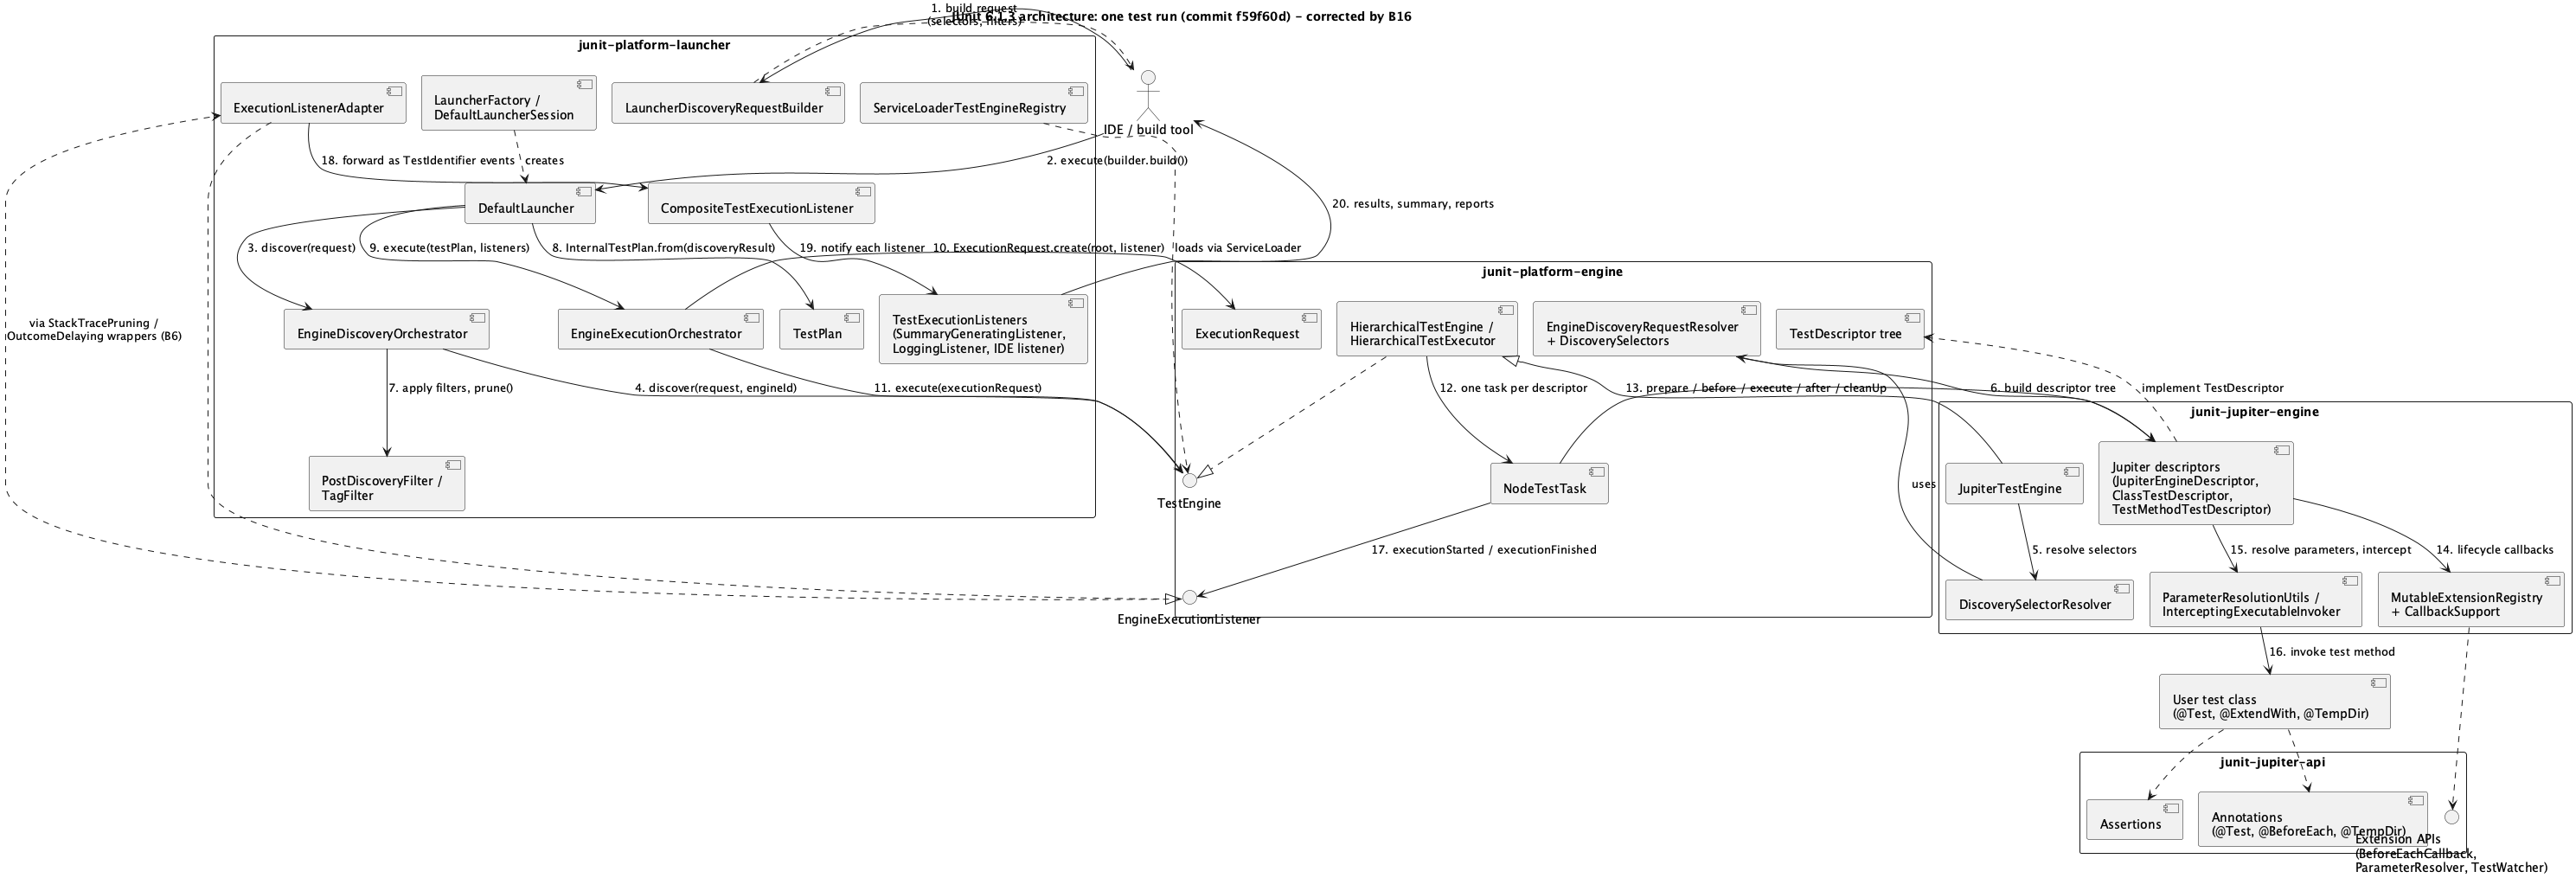
\includegraphics[height=0.82\textheight,width=\linewidth,keepaspectratio]{Part1/architecture/architecture.png}
\end{frame}

\begin{frame}{Part 1: patterns found at the baseline}
\begin{columns}
\column{0.5\textwidth}
\begin{tabular}{@{}lr@{}}\toprule Pattern & Instances\\\midrule
Strategy & 10\\ Adapter & 5\\ Observer & 5\\ Decorator & 4\\ Template Method & 3\\
Composite & 2\\ Command & 2\\ Null Object & 2\\ Chain of Responsibility & 1\\ Factory Method & 1\\\midrule
\textbf{Total} & \textbf{35}\\\bottomrule\end{tabular}
\column{0.48\textwidth}
\begin{itemize}
\item 10 pattern types, 35 instances
\item 76 concrete participant classes, 152 unique symbols
\item 25 rejected, 8 uncertain candidates
\item Composite rule: combine children of the same interface \emph{and} merge their answers
\item 102 LLM claims verified
\end{itemize}
\end{columns}
\end{frame}

\begin{frame}{Example: A1 Test Descriptor Tree (Composite)}
\centering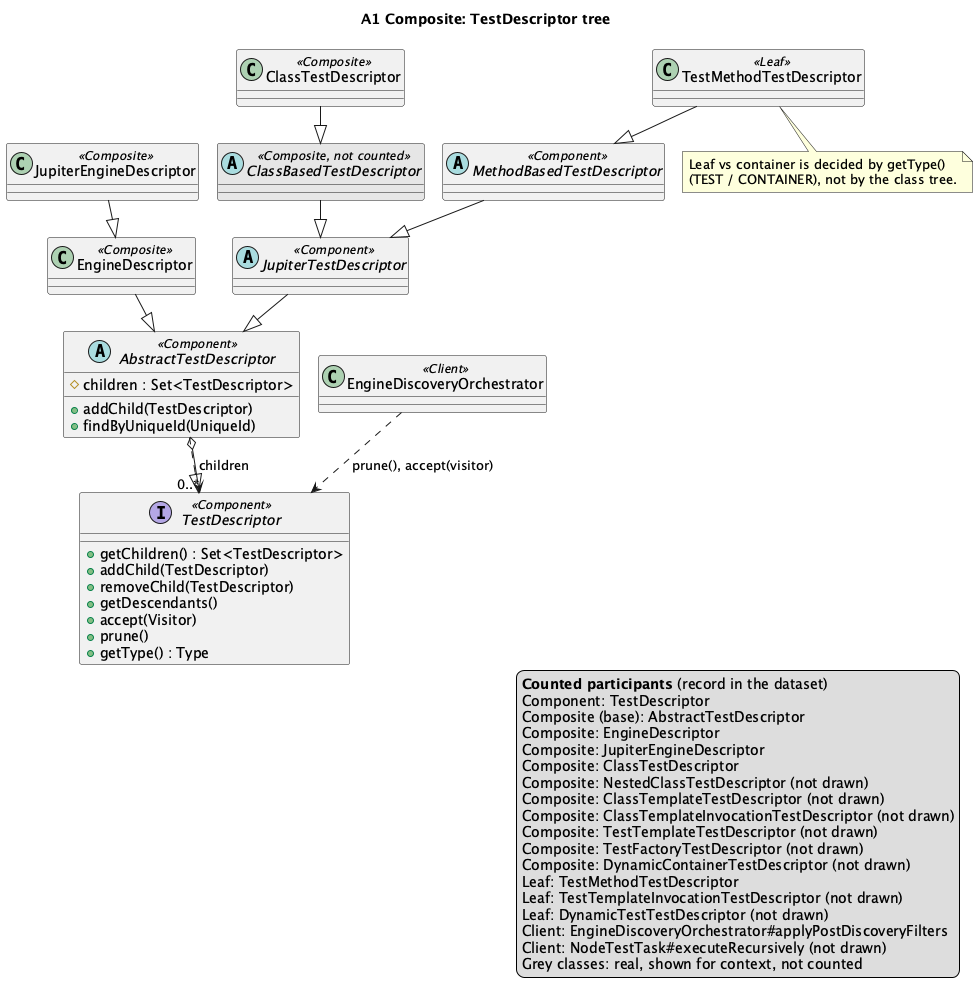
\includegraphics[height=0.82\textheight,width=\linewidth,keepaspectratio]{Part1/uml/png/A1.png}
\end{frame}

\begin{frame}{Part 2: three changes}
\small
\begin{tabular}{@{}L{0.19\linewidth}L{0.32\linewidth}L{0.19\linewidth}L{0.2\linewidth}@{}}\toprule
Change & What & Kind & Refactoring\\\midrule
CH03 filter policy & \texttt{off|exclude|only} over tags/methods from \texttt{junit-platform.properties} & implementation change & preparatory Extract Method\\
CH01 summary listener & per-class table + slowest tests, ServiceLoader, off by default & existing extension point & Extract Method \texttt{count()} (CCN 10 $\to$ 4)\\
CH02 \texttt{@ManagedResource} & create/inject/destroy any resource, per class or per test & existing extension points only & none (no existing code changed)\\\bottomrule
\end{tabular}
\vspace{6pt}
\begin{itemize}
\item JUnit suites after every commit: launcher 382 $\to$ 397, platform 2452 $\to$ 2467, Jupiter 3381 $\to$ 3388, 0 failures
\item Mutation checks: the new tests fail when the feature is removed
\end{itemize}
\end{frame}

\begin{frame}{Pattern evolution}
\begin{tabular}{@{}lrrl@{}}\toprule
Snapshot & Instances & Concrete & Change\\\midrule
Original & 35 & 76 & baseline\\
After CH03 & 35 & 78 & A2 Composite, A3 Strategy \emph{extended}\\
After CH01 & 35 & 79 & C1 Observer \emph{extended}\\
After CH02 & 37 & 81 & D3 \emph{extended}; N1 Strategy, N2 Adapter \emph{new}\\\bottomrule
\end{tabular}
\vspace{8pt}
\begin{itemize}
\item No pattern replaced or removed: changes plug into existing Strategy/Observer points
\item LLM corrections: no ``enum Strategy'' (D1-18), not a Long Method (D1-20), Holder \emph{is} an Adapter (D1-22)
\end{itemize}
\end{frame}

\begin{frame}{N2: Managed Resource Holder (Adapter, new in CH02)}
\centering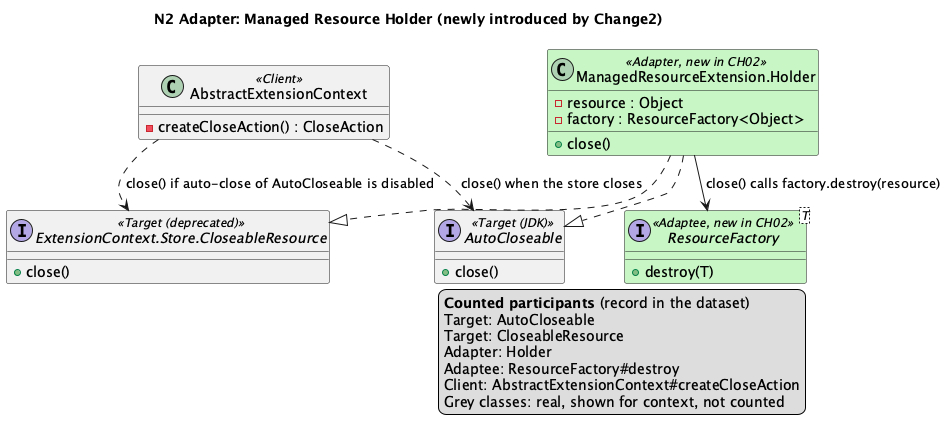
\includegraphics[height=0.82\textheight,width=\linewidth,keepaspectratio]{Part2/uml/png/N2.png}
\end{frame}

\begin{frame}{Part 3: all 10 pattern types in four languages}
\small
\begin{columns}
\column{0.46\textwidth}
{\footnotesize\begin{tabular}{@{}lrrr@{}}\toprule
Language & Mean LOC & Max CC & Median ms\\\midrule
Java & 138.0 & 6--22 & 32.0--36.8\\
Python & 86.5 & 6--22 & 21.0--21.8\\
JavaScript & 102.0 & 5--17 & 91.4--93.2\\
C++ & 142.1 & 6--24 & 4.8--5.9\\
\bottomrule\end{tabular}}

\vspace{4pt}\footnotesize 40 programs; ranges over the 10 problems.
\column{0.52\textwidth}
\begin{itemize}
\item One problem per type, each modelled on a Part 1 instance (A1, A3, B1, B2, B7, B9, C1, C7, D9, D10)
\item Same input, byte-identical output; 110/110 commands pass; every runner 3/3; C++ clean under ASan/UBSan, 0 leaks
\item Java/C++ state contracts in types; Python/JS rely on duck typing
\item C++ makes ownership explicit (\texttt{unique\_ptr}); time is runtime start-up
\end{itemize}
\end{columns}
\end{frame}

\begin{frame}{AI use and verification}
\begin{itemize}
\item claude.ai: analysis prompts, 2 Part 3 problems; Claude Code: Part 2 code, 8 Part 3 problems, scripts (all in \texttt{data/llm.csv})
\item Verified claims: Part 1: 102, Part 2: 22, Part 3: 16 -- with corrections recorded, not hidden
\item Generated code accepted only after JUnit's own suites, mutation checks and demos on the official vs evolved jar
\end{itemize}
\end{frame}

\begin{frame}{Findings}
\begin{itemize}
\item JUnit is built on a few patterns used many times: Strategy for every policy, Observer for events, Adapter between APIs, Composite for the test tree
\item These extension points made two of three changes possible without touching JUnit's code
\item Refactoring helped where the smell was real (CCN 10 $\to$ 4) and changed little where it was preparatory
\item Limits: four modules, production code only, single-machine timings
\end{itemize}
\end{frame}

\end{document}
